%!TEX root = ../template.tex
%%%%%%%%%%%%%%%%%%%%%%%%%%%%%%%%%%%%%%%%%%%%%%%%%%%%%%%%%%%%%%%%%%%%
%% chapter3.tex
%% NOVA thesis document file
%%
%% Chapter with a short latex tutorial and examples
%%%%%%%%%%%%%%%%%%%%%%%%%%%%%%%%%%%%%%%%%%%%%%%%%%%%%%%%%%%%%%%%%%%%

\typeout{NT FILE chapter3.tex}%

\chapter{State Of The Art}
\label{cha:State_Of_The_Art}

\section{Certified Compilers}
\label{sec:Certified_Compilers}

\subsection{CompCert}
\label{sec:CompCert}

\subsection{CakeML}
\label{sec:CakeML}

%% https://github.com/CakeML/cakeml/blob/master/how-to.md

%%lets terminam com end e nao esta a acontecer na extracao
%%literais boleanos comecam com letra grande
%%cakeml nao suportam loops sem ser recursivos
%%Ref e com letra grande
%%datatypes ficam todos mal feitos e trocados
%%operacoes com arrays nao funciona bem na traducao
%%expections sao definidas fora da funcao

\section{Pipeline}
\label{sec:Pipeline}

Some parts of the verification pipeline have already been implemented or require only minor adjustments to meet their 
objectives. As we know, \cameleer provides translation of \ocaml code annotated with \gospel specifications into \whyml :

\begin{figure}[H]
    \centering
    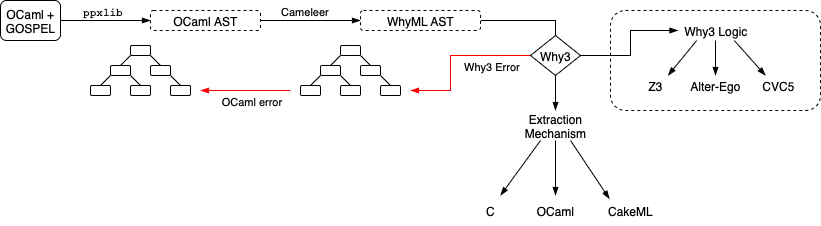
\includegraphics[width=\linewidth]{images/Cameleer.png}
    \caption{\ocaml to \whyml pipeline with \cameleer}
\end{figure}

The extraction process does not require the correctness of the code to be proven. This may lead to potentially incorrect \ocaml 
programs to be extracted to \cml. Additionally, it is not designed to prevent users from extracting code even if the \gospel 
specifications can not guarantee correctness.

%%Processo de extracao nao esta ligado ao facto de um exemplo ja ter sido provado ou nao, pode potencialmente 
%%levar a gerar codigo cakeml nao correto

By modifying the extraction process in \whythree to check if the proof has been discharged we can provide better correctness 
guarantees because the generated \cml code will comply to the specification. Due to differences in syntax and features that 
have no direct equivalents in \cml, we must also include some kind of error message for failures in extraction, for instance 
the lack of support for while and for loops.

The goal of this work is to expand the currently available pipeline of translating code from \ocaml with \gospel specifications 
into \whyml, where it can be verified using the various automated provers available in Why3. One of our goals is to achieve 
a more robust extraction mechanism with the ideas as previously discussed. Moreover, we ought to provide a new tool that 
translates compilable \cml programs into \ocaml equivalents that can be specified afterwards with \gospel so that one may prove 
their correctness in \cameleer.

\begin{figure}[H]
    \centering
    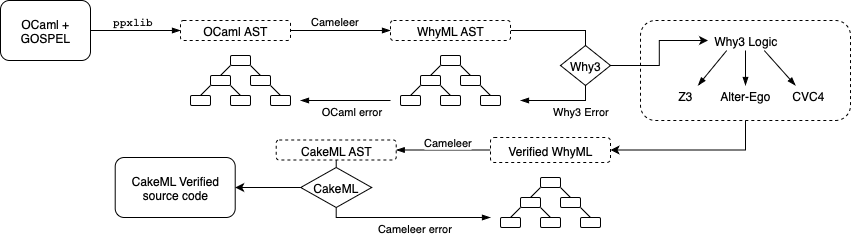
\includegraphics[width=\linewidth]{images/Goal_Pipeline.png}
    \caption{Goal pipeline}
\end{figure}



%%existe extracao cameleer para whyml, de whyml para cakeml, whyml para ocaml64